\documentclass{article}
\usepackage{pgfplots}
\pgfplotsset{compat=1.16}

\begin{document}

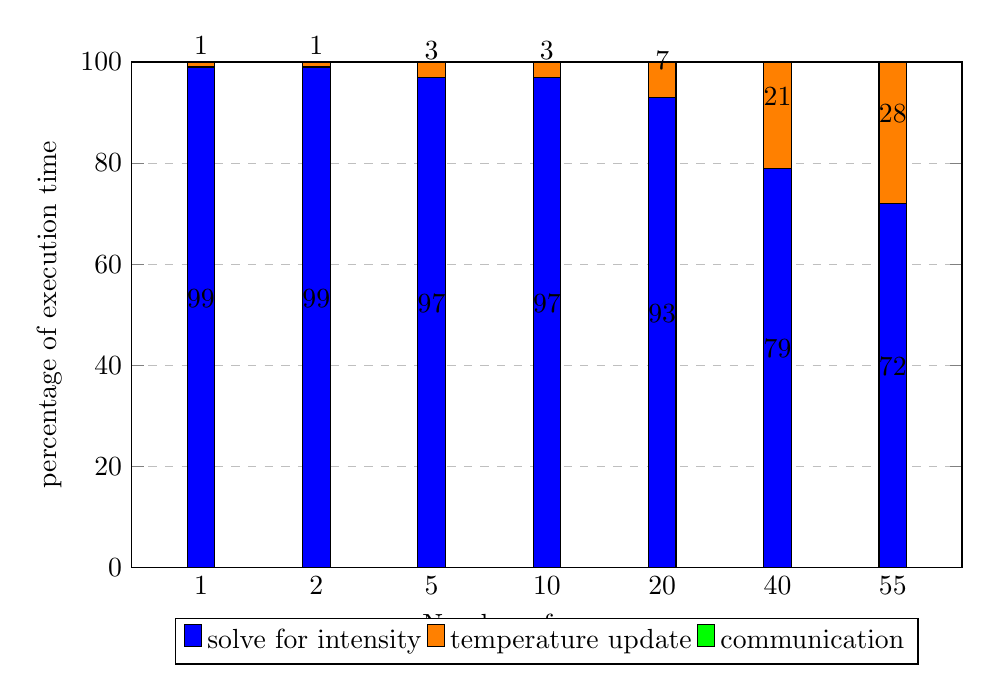
\begin{tikzpicture}
    \begin{axis}[
        ybar stacked,
        width=\textwidth,
        height=8cm,
        xlabel={Number of processes},
        ylabel={percentage of execution time},
        symbolic x coords={1, 2, 5, 10, 20, 40, 55},
        xtick=data,
        nodes near coords,
        nodes near coords align={vertical},
        legend style={at={(0.5,-0.1)}, anchor=north,legend columns=-1},
        ymin=0, ymax=100,
        ymajorgrids=true,
        grid style=dashed,
    ]
    
    \addplot[fill=blue] coordinates {(1,99) (2,99) (5,97) (10,97) (20,93) (40,79) (55,72)};
    \addplot[fill=orange] coordinates {(1,1) (2,1) (5,3) (10,3) (20,7) (40,21) (55,28)};
    \addplot[fill=green] coordinates {(1,0) (2,0) (5,0) (10,0) (20,0) (40,21) (55,28)};

    \legend{solve for intensity, temperature update, communication}
    
    \end{axis}
\end{tikzpicture}

\end{document}